\documentclass[11pt]{article}
\usepackage{fullpage}
\usepackage{amsthm}
\usepackage{amsmath} \usepackage{amssymb}
\usepackage{graphicx}

\graphicspath{ {./imgs/} }

\setlength{\parindent}{0pt}

\title{Graphics (CO317)}
\author{Michael Tsang}

\newtheorem{defn}{Definition}
\newtheorem{eg}{Example}
\newtheorem{theo}{Theorem}
\newtheorem{lem}{Lemma}

\begin{document}

\maketitle

\section{Projections and Transformations}
\subsection{Device Independence}
Device dependent graphics primitive methods are:
\begin{verbatim}
  SetPixel(XCoord, YCoord, Colour);
  DrawLine(xs, ys, xf, yf);
\end{verbatim}

\textbf{Device independence} allows us to resize or transport a picture to a different operating system, and have it fit exactly in the window where we place it.
We define a \textbf{world coordinate system} when drawing objects, typically it will use a method of the kind:
\begin{verbatim}
  SetWindowCoords(Wxmin, Wymin, Wxmax, Wymax);
\end{verbatim}

The units of these arguments will depend on that application.
The application uses drawing primitives and these units to convert their numeric values to pixels, before the image is rendered on the screen.

In order to implement a world coordinate system, we need to be able to translate between world coordinates and the device or pixel coordinates.
We first find out the pixel coordinates of the window:
\begin{verbatim}
  GetWindowPixelCoords(Vxmin, Vymin, Vxmax, Vymax);
\end{verbatim}

\begin{figure}[h]
  \caption{World coordinate window against viewport on the screen.}
  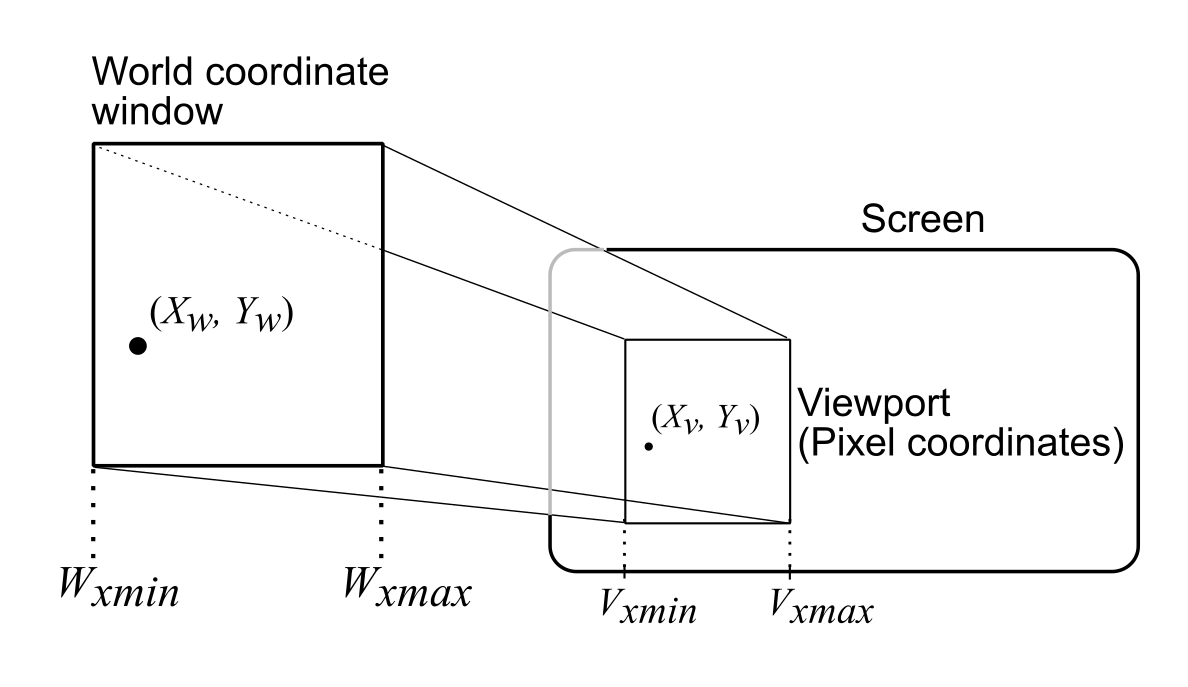
\includegraphics[scale=0.4]{normalisation}
  \centering
\end{figure}

We then perform normalisation to compute the pixel coordinates from the world coordinates, using simple ratios.
For the $x$ direction:
\[
  \frac{X_w - W_{xmin}}{W_{xmax} - W_{xmin}} = \frac{X_v - V_{xmin}}{V_{xmax} - V_{xmin}}
\]
\[
  X_v = \frac{(X_w - W_{xmin})(V_{xmax} - V_{xmin})}{W_{xmax} - W_{xmin}} + V_{xmin}
\]

With a similar expression for $y$.

From the known values, we can form a simple pair of linear equations:
\begin{align*}
  X_v &= AX_w + B \\
  Y_v &= CY_w + D
\end{align*}

If the window is moved or resized, we must re-calculate the constants $A, B, C, D$.

\subsection{Representing Planar Polygons}
Most graphical scenes and objects are built out of planar polyhedra, three-dimensional objects whose faces are all planar polygons (\textbf{faces} or \textbf{facets}).
To describe objects made of polygons, we need the \textbf{locations} of the vertices and their \textbf{topology}.

\begin{itemize}
  \item Numerical Data - 3D coordinates of vertices.
  \item Topological Data - what is connected to what.
\end{itemize}

\begin{figure}[h]
  \caption{Data for a polygon.}
  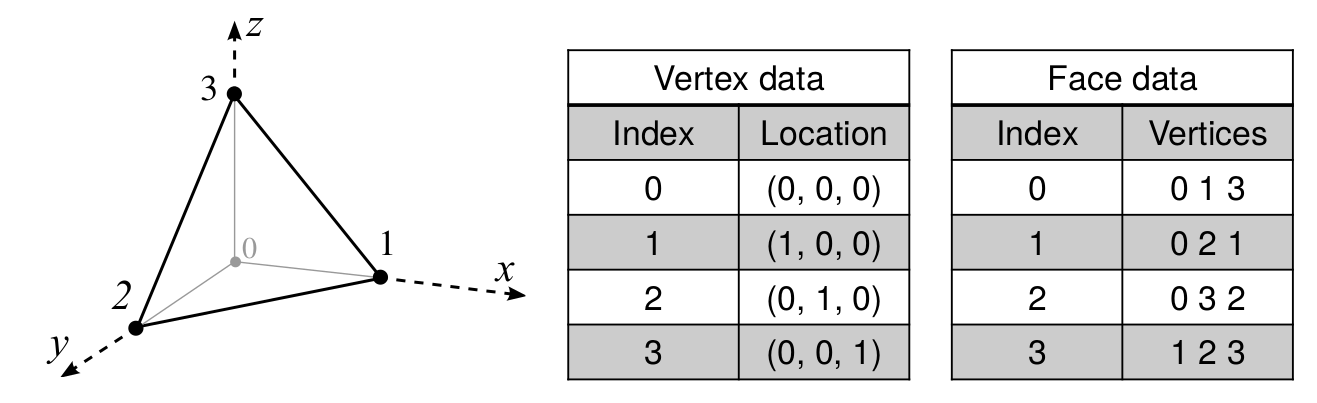
\includegraphics[scale=0.3]{polygon}
  \centering
\end{figure}

\subsection{Projections of Wire-Frame Models}
A \textbf{projection} transforms an $n$-dimensional space into an $m$-dimensional space, where $m < n$.
When projecting an object onto a surface, we first select a viewpoint then define \textit{projectors} or lines which join each vertex of the object to the viewpoint.
Where the projector intersects with the surface is defined as the projection of the corresponding vertex in the object.

The most common projections for viewing 3D scenes use a plane for the projection surface and straight lines for the projectors, these are \textbf{planar geometric projections}.
\textbf{Wire frame} models simply include points and lines, to render such a representation we need to specify only which edges join which points.
Other forms of rendering need to define the object faces.

There are two commons types of planar geometric projection:
\begin{itemize}
  \item \textbf{Parallel projection} - parallel projectors.
  \item \textbf{Perspective projection} - projectors pass through a single point (\textit{viewpoint}).
\end{itemize}

We first make some assumptions:
\begin{itemize}
  \item The viewpoint is at $z = - \infty$.
  \item The plane of projection is $z = 0$ (we can use coordinate transformations in 3D to make it so).
\end{itemize}

\subsection{Orthographic Projections}
In parallel projection, all projectors have the same direction $d$, and the viewpoint is considered to be at infinity.
For a vertex $V = (V_x, V_y, V_z)^\intercal$:
\[
  P = V + \mu d
\]

A special case is \textbf{orthographic projection}, where the projectors are perpendicular to the projection plane.
This means:
\[
  d = 
  \begin{pmatrix}
    0 \\
    0 \\
    -1
  \end{pmatrix}
\]

\begin{figure}[h]
  \caption{Parallel projection.}
  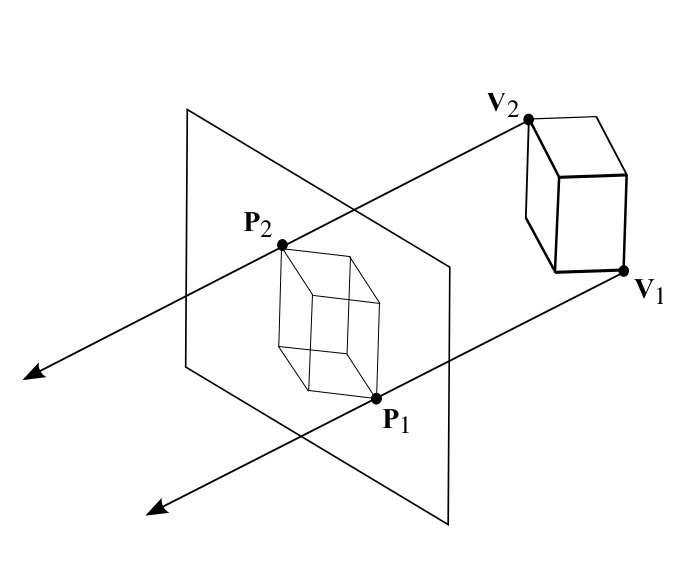
\includegraphics[scale=0.3]{parallel}
  \centering
\end{figure}

Which gives the Cartesian equations for each component:
\begin{align*}
  P_x &= V_x  & P_y &= V_y & P_z &= V_z - \mu
\end{align*}
Note that since $z = 0$, then $P_z = 0$.

This means we simply take the $x$ and $y$ coordinates:
\[
  P =
  \begin{pmatrix}
    V_x \\
    V_y \\
    0
  \end{pmatrix}
\]

\subsection{Perspective Projections}
Orthographic projections are fine in cases where we do not care about depth.
In \textbf{perspective projection}, all the projectors pass through one point in space, the \textit{centre of projection}.
If the centre of projection is on the opposite side of the plane of projection compared to the 3D object, the orientation of the image is the same as the object.
Otherwise if thecentre is between the plane and the object, the image is inverted.

\begin{figure}[h]
  \caption{Perspective projection where the viewpoint is on the opposite side of the object.}
  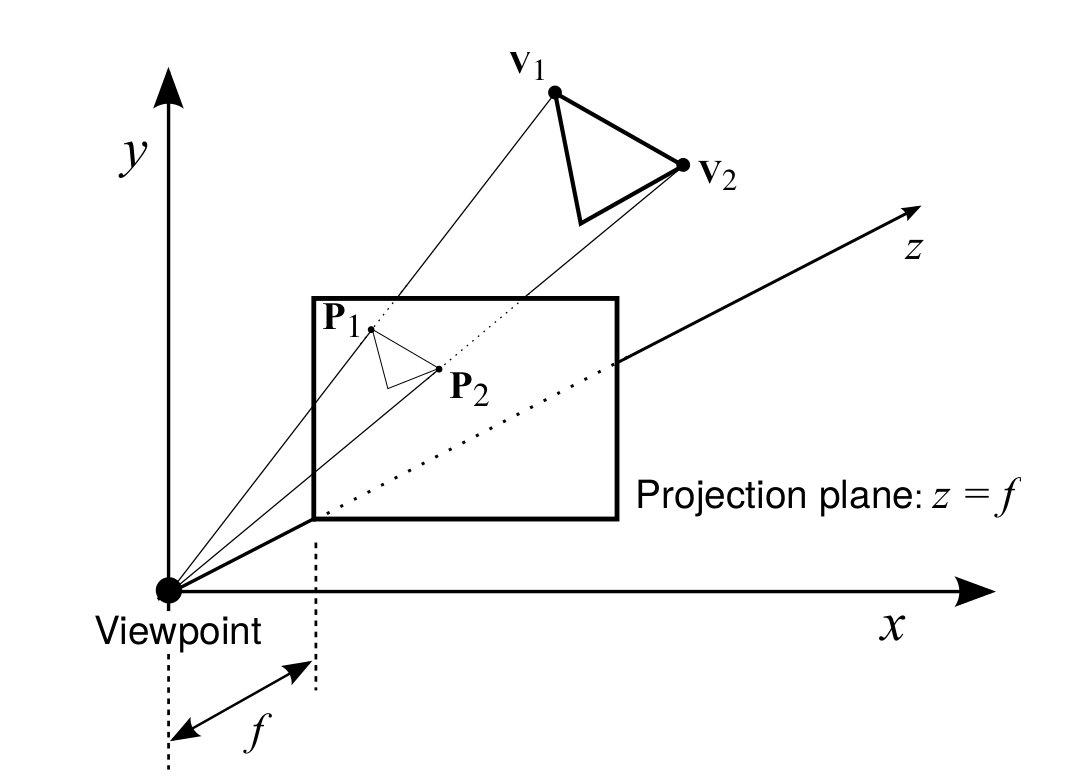
\includegraphics[scale=0.3]{perspective}
  \centering
\end{figure}

We first make two assumptions:
\begin{itemize}
  \item The centre of projection is at the origin.
  \item The projection plane is placed at a constant $z$ value, $z = f$.
\end{itemize}

The perspective projector equation from vertex $V$ is:
\[
  P = \mu V
\]

It follows that since $z = f$, then $f = \mu V_z$, and $\mu_p = f / V_z$.

This means:
\begin{align*}
  P_x = \mu_p V_x = \frac{fV_x}{V_z} && P_y = \mu_p V_y = \frac{fV_y}{V_z}
\end{align*}

We call $\mu_p$ the \textit{foreshortening} factor, if the object moves further away then $V_z$ increases and the image becomes smaller.

\subsection{Space Transformations}
Graphics scenes are defined in a particular coordinate system but we want to be able to view it at any point of our choosing.

We may also want to transform for other purposes:
\begin{itemize}
  \item Animating objects.
  \item Multiple instances.
  \item Reflections and other special effects.
\end{itemize}

In order to still be able to use canonical projection, we need to transform the coordinates of the scene so that the view direction is along the $z$-axis and the viewpoint at the origin.
That is, we want to change the coordinates of every point in the scene such that some chosen viewpoint $C$ becomes the origin, and the chosen view direction $d$ becomes the $z$-axis.
Transformation matricies can be used for nearly all simple transformations, except for translation using normal Cartesian coordinates.
We thus introduce \textbf{homogeneous coordinates}.

\subsubsection{Homogeneous Coordinates}
To express a point in homogeneous coordinates, we introduce a fourth coordinate (or \textit{ordinate}):
\[
  P =
  \begin{pmatrix}
    p_x \\
    p_y \\
    p_z \\
    s
  \end{pmatrix}
\]

The fourth ordinate is a scale factor, we use it to convert back to Cartesian form by dividing it into the other ordinates.
\[
  (p_x, p_y, p_z, s) \Leftrightarrow (\frac{p_x}{s}, \frac{p_y}{s}, \frac{p_z}{s})
\]
In most cases $s$ is $1$.

\subsubsection{Translation}
To represent translation:
\[
  \begin{pmatrix}
    1 & 0 & 0 & t_x \\
    0 & 1 & 0 & t_y \\
    0 & 0 & 1 & t_z \\
    0 & 0 & 0 & 1
  \end{pmatrix}
  \begin{pmatrix}
    p_x \\
    p_y \\
    p_z \\
    1
  \end{pmatrix}
  =
  \begin{pmatrix}
    p_x + t_x \\
    p_y + t_y \\
    p_z + t_z \\
    1
  \end{pmatrix}
\]

The inverse is:
\[
  \begin{pmatrix}
    1 & 0 & 0 & -t_x \\
    0 & 1 & 0 & -t_y \\
    0 & 0 & 1 & -t_z \\
    0 & 0 & 0 & 1
  \end{pmatrix}
\]

\subsubsection{Scaling}
To represent scaling:
\[
  \begin{pmatrix}
    s_x & 0 & 0 & 0 \\
    0 & s_y & 0 & 0 \\
    0 & 0 & s_z & 0 \\
    0 & 0 & 0 & 1
  \end{pmatrix}
  \begin{pmatrix}
    p_x \\
    p_y \\
    p_z \\
    1
  \end{pmatrix}
  =
  \begin{pmatrix}
    s_xp_x \\
    s_yp_y \\
    s_zp_z \\
    1
  \end{pmatrix}
\]

The inverse is:
\[
  \begin{pmatrix}
    1/s_x & 0 & 0 & 0 \\
    0 & 1/s_y & 0 & 0 \\
    0 & 0 & 1/s_z & 0 \\
    0 & 0 & 0 & 1
  \end{pmatrix}
\]


\subsubsection{Combining Transformations}
To combine transformations, we can multiply out their matrices and apply the transformation with the resultant matrix.

\begin{figure}[h]
  \caption{Importance of the order of transformations.}
  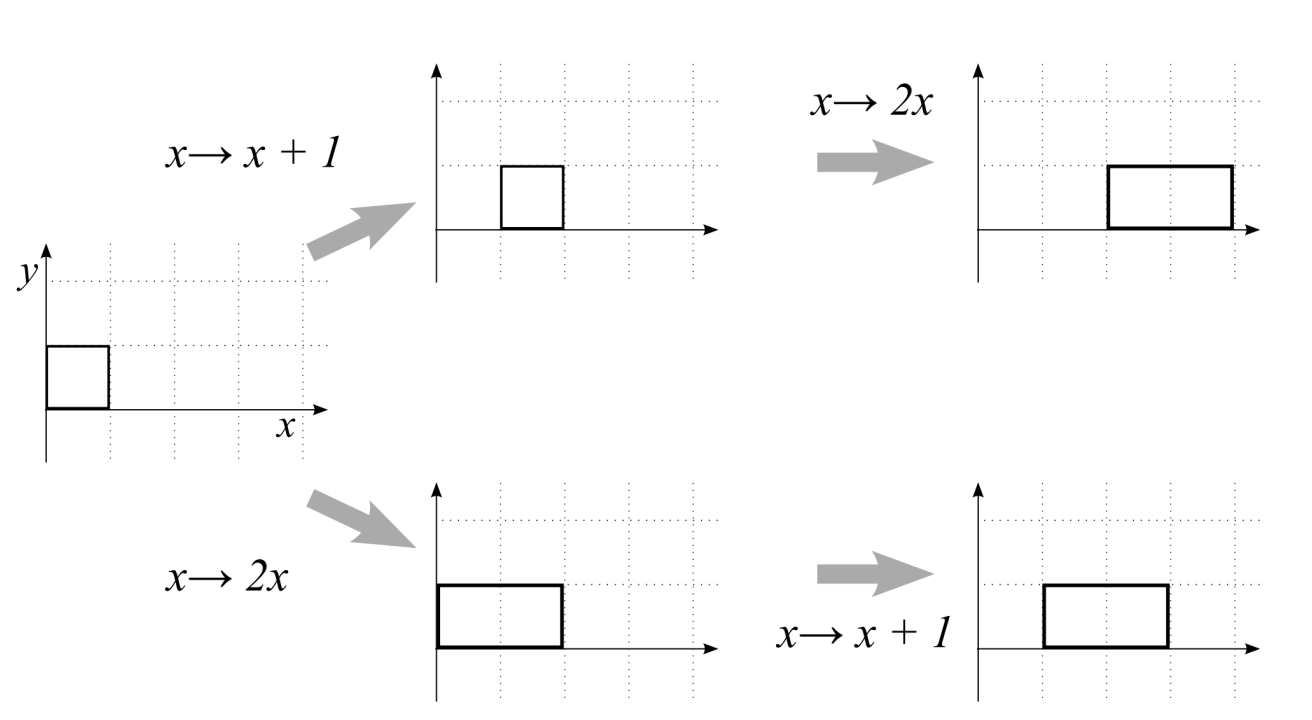
\includegraphics[scale=0.2]{combining}
  \centering
\end{figure}

Transformations are not necessarily commutative, it is important that they are carried out in the correct order.

\subsubsection{Rotation}
To define rotation we need an axis and an angle.
Matrices for rotation around the three cartesian axes are:
\begin{align*}
  \mathcal{R}_x &=
  \begin{pmatrix}
    1 & 0 & 0 & 0 \\
    0 & \cos \theta & -\sin \theta & 0 \\
    0 & \sin \theta & \cos \theta & 0 \\
    0 & 0 & 0 & 1
  \end{pmatrix} \\
  \mathcal{R}_y &=
  \begin{pmatrix}
    \cos \theta & 0 & \sin \theta & 0 \\
    0 & 1 & 0 & 0 \\
    -\sin \theta & 0 & \cos \theta & 0 \\
    0 & 0 & 0 & 1
  \end{pmatrix} \\
  \mathcal{R}_z &=
  \begin{pmatrix}
    \cos \theta &  -\sin \theta & 0 & 0 \\
    \sin \theta & \cos \theta & 0 & 0 \\
    0 & 0 & 1 & 0 \\
    0 & 0 & 0 & 1
  \end{pmatrix}
\end{align*}

\begin{figure}[h]
  \caption{Rotation of a coordinate ($z$-axis goes into the page).}
  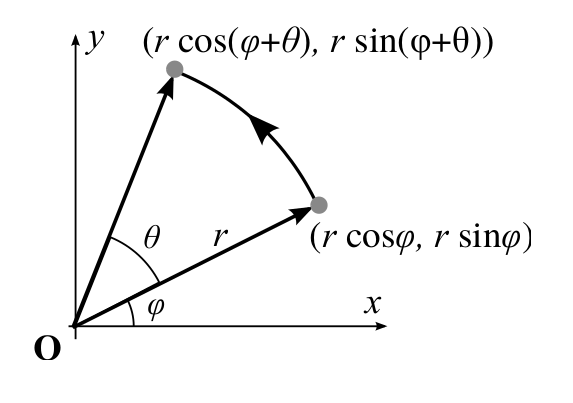
\includegraphics[scale=0.3]{deriverotate}
  \centering
\end{figure}

An example for how we derive $\mathcal{R}_z$ is as follows:
\[
  \begin{pmatrix}
    x \\
    y
  \end{pmatrix}
  =
  \begin{pmatrix}
    r \cos \varphi \\
    r \sin \varphi
  \end{pmatrix}
\]
\begin{align*}
  \begin{pmatrix}
    r \cos (\varphi + \theta) \\
    r \sin (\varphi + \theta)
  \end{pmatrix}
  &=
  \begin{pmatrix}
    r \cos \varphi \cos \theta - r \sin \varphi \sin \theta \\
    r \cos \varphi \sin \theta + r \sin \varphi \cos \theta
  \end{pmatrix} \\
  &=
  \begin{pmatrix}
    x \cos \theta - y \sin \theta \\
    x \sin \theta + y \cos \theta
  \end{pmatrix} \\
  &=
  \begin{pmatrix}
    \cos \theta & - \sin \theta \\
    \sin \theta & \cos \theta
  \end{pmatrix}
  \begin{pmatrix}
    x \\
    y
  \end{pmatrix}
\end{align*}

The $2 \times 2$ matrix is the same as the upper left corner of the matrix $\mathcal{R}_z$.

This assumes a left had axis system.
\begin{itemize}
  \item Rotation is \textbf{anti-clockwise} when looking along the axis of rotation.
  \item Rotation is \textbf{clockwise} when looking back towards the origin from the positive side of the axis.
\end{itemize}

To invert rotation, we rotate through an angle of $- \theta$, and note the follow relations:
\begin{align*}
  \cos(-\theta) &= \cos(\theta) & \sin(-\theta)=-\sin(\theta)
\end{align*}

Then for example:
\[
  \mathcal{R}_z(-\theta) = 
  \begin{pmatrix}
    \cos \theta & \sin \theta & 0 & 0 \\
    - \sin \theta & \cos \theta & 0 & 0 \\
    0 & 0 & 1 & 0 \\
    0 & 0 & 0 & 1
  \end{pmatrix}
\]

\end{document}
